\paragraph{Second development round.}

Round 2 keeps the same twenty documents, compiler, reward, budget,
and expansion check. Prompts add readable entity names and explain
property direction, historical roles, and absent versus conflicting
evidence. Forty more requests complete with zero transport failures.
Thirty-eight responses pass the fixed parser. They yield 243 type
rules, 14 source-support rules, and zero source-contradiction rules.

Acquire-then-repair and repair-when-feasible both reach 95.69\% reference
F1, compared with 94.42\% for stop. Each removes seven of 31 injected
items and loses zero reference facts. All seven removals use type rules.
The source-repair check ends the two-round study.

The compiler rejects 120 type candidates in round 1 and 257 in round 2
that copy \texttt{allowed or forbidden} instead of choosing one kind.
Both rounds use the fixed parser. The logs retain round 1 reference
losses and round 2 source-rule results.

\begin{figure*}[t]
\centering
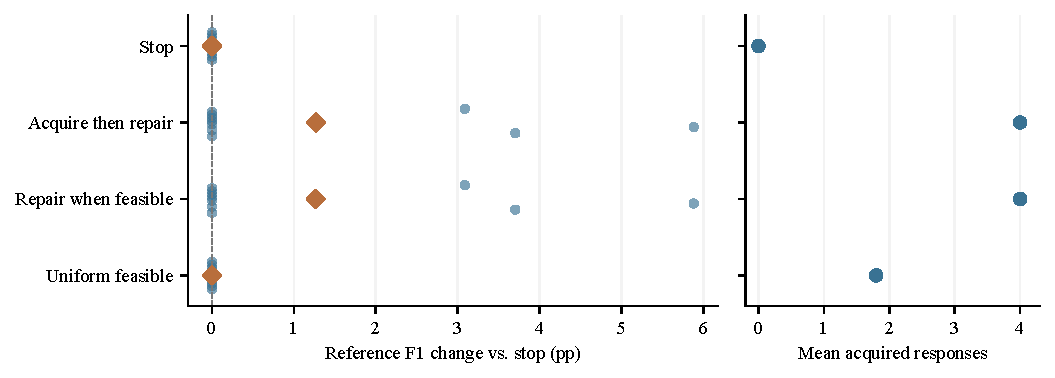
\includegraphics[width=0.94\textwidth]{figure/experiments/docred_source_pilot_round2.pdf}
\caption{Round 2 on the same ten development pairs. Both full schedules reach 95.69\% mean F1 and keep every reference fact. Seven removals use type rules.}
\label{fig:docred_source_round2}
\end{figure*}
